\documentclass[tikz]{standalone}
\usepackage{amsmath,amssymb}
\usepackage{tikz}
\usetikzlibrary{
	shapes,
	snakes,
	calc,
	decorations,
	decorations.markings,
	decorations.text,
	decorations.pathreplacing}
	
\begin{document}
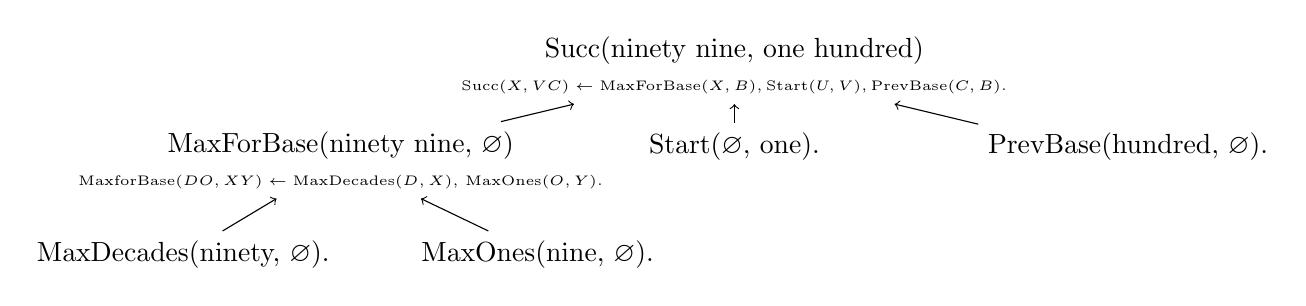
\begin{tikzpicture}[scale=1,auto,every text node part/.style={align=center}]
  % Parse Tree
  \node (S0) at (0,2.4) {Succ(ninety nine, one hundred)\\
    \tiny$\text{Succ}(X,VC) \leftarrow \text{MaxForBase}(X,B), \text{Start}(U,V), \text{PrevBase}(C,B).$};
  \node (MFB1) at (-5,1.2) {MaxForBase(ninety nine, $\varnothing$)\\
    \tiny$\text{MaxforBase}(DO,XY) \leftarrow \text{MaxDecades}(D,X),\,\text{MaxOnes}(O,Y).$};
  \node (S1) at (0,1.2) {Start($\varnothing$, one).\\};
  \node (PB1) at (5,1.2) {PrevBase(hundred, $\varnothing$).\\};
  \node (MD2) at (-7,0) {MaxDecades(ninety, $\varnothing$).};
  \node (MO2) at (-2.5,0) {MaxOnes(nine, $\varnothing$).};

  \draw [<-] (S0)     to (MFB1);
  \draw [<-] (S0)     to (S1);
  \draw [<-] (S0)     to (PB1);
  \draw [<-] (MFB1)  to (MD2);
  \draw [<-] (MFB1)  to (MO2);
\end{tikzpicture}
\end{document}
